\documentclass[twoside]{book}

% Packages required by doxygen
\usepackage{fixltx2e}
\usepackage{calc}
\usepackage{doxygen}
\usepackage[export]{adjustbox} % also loads graphicx
\usepackage{graphicx}
\usepackage[utf8]{inputenc}
\usepackage{makeidx}
\usepackage{multicol}
\usepackage{multirow}
\PassOptionsToPackage{warn}{textcomp}
\usepackage{textcomp}
\usepackage[nointegrals]{wasysym}
\usepackage[table]{xcolor}

% NLS support packages
\usepackage[brazil]{babel}
% Font selection
\usepackage[T1]{fontenc}
\usepackage[scaled=.90]{helvet}
\usepackage{courier}
\usepackage{amssymb}
\usepackage{sectsty}
\renewcommand{\familydefault}{\sfdefault}
\allsectionsfont{%
  \fontseries{bc}\selectfont%
  \color{darkgray}%
}
\renewcommand{\DoxyLabelFont}{%
  \fontseries{bc}\selectfont%
  \color{darkgray}%
}
\newcommand{\+}{\discretionary{\mbox{\scriptsize$\hookleftarrow$}}{}{}}

% Page & text layout
\usepackage{geometry}
\geometry{%
  a4paper,%
  top=2.5cm,%
  bottom=2.5cm,%
  left=2.5cm,%
  right=2.5cm%
}
\tolerance=750
\hfuzz=15pt
\hbadness=750
\setlength{\emergencystretch}{15pt}
\setlength{\parindent}{0cm}
\setlength{\parskip}{3ex plus 2ex minus 2ex}
\makeatletter
\renewcommand{\paragraph}{%
  \@startsection{paragraph}{4}{0ex}{-1.0ex}{1.0ex}{%
    \normalfont\normalsize\bfseries\SS@parafont%
  }%
}
\renewcommand{\subparagraph}{%
  \@startsection{subparagraph}{5}{0ex}{-1.0ex}{1.0ex}{%
    \normalfont\normalsize\bfseries\SS@subparafont%
  }%
}
\makeatother

% Headers & footers
\usepackage{fancyhdr}
\pagestyle{fancyplain}
\fancyhead[LE]{\fancyplain{}{\bfseries\thepage}}
\fancyhead[CE]{\fancyplain{}{}}
\fancyhead[RE]{\fancyplain{}{\bfseries\leftmark}}
\fancyhead[LO]{\fancyplain{}{\bfseries\rightmark}}
\fancyhead[CO]{\fancyplain{}{}}
\fancyhead[RO]{\fancyplain{}{\bfseries\thepage}}
\fancyfoot[LE]{\fancyplain{}{}}
\fancyfoot[CE]{\fancyplain{}{}}
\fancyfoot[RE]{\fancyplain{}{\bfseries\scriptsize Gerado por Doxygen }}
\fancyfoot[LO]{\fancyplain{}{\bfseries\scriptsize Gerado por Doxygen }}
\fancyfoot[CO]{\fancyplain{}{}}
\fancyfoot[RO]{\fancyplain{}{}}
\renewcommand{\footrulewidth}{0.4pt}
\renewcommand{\chaptermark}[1]{%
  \markboth{#1}{}%
}
\renewcommand{\sectionmark}[1]{%
  \markright{\thesection\ #1}%
}

% Indices & bibliography
\usepackage{natbib}
\usepackage[titles]{tocloft}
\setcounter{tocdepth}{3}
\setcounter{secnumdepth}{5}
\makeindex

% Hyperlinks (required, but should be loaded last)
\usepackage{ifpdf}
\ifpdf
  \usepackage[pdftex,pagebackref=true]{hyperref}
\else
  \usepackage[ps2pdf,pagebackref=true]{hyperref}
\fi
\hypersetup{%
  colorlinks=true,%
  linkcolor=blue,%
  citecolor=blue,%
  unicode%
}

% Custom commands
\newcommand{\clearemptydoublepage}{%
  \newpage{\pagestyle{empty}\cleardoublepage}%
}

\usepackage{caption}
\captionsetup{labelsep=space,justification=centering,font={bf},singlelinecheck=off,skip=4pt,position=top}

%===== C O N T E N T S =====

\begin{document}

% Titlepage & ToC
\hypersetup{pageanchor=false,
             bookmarksnumbered=true,
             pdfencoding=unicode
            }
\pagenumbering{roman}
\begin{titlepage}
\vspace*{7cm}
\begin{center}%
{\Large Projeto -\/ I\+CC \\[1ex]\large 1 }\\
\vspace*{1cm}
{\large Gerado por Doxygen 1.8.11}\\
\end{center}
\end{titlepage}
\clearemptydoublepage
\tableofcontents
\clearemptydoublepage
\pagenumbering{arabic}
\hypersetup{pageanchor=true}

%--- Begin generated contents ---
\chapter{Índice das Estruturas de Dados}
\section{Estruturas de Dados}
Aqui estão as estruturas de dados, uniões e suas respectivas descrições\+:\begin{DoxyCompactList}
\item\contentsline{section}{\hyperlink{structdbEdge}{db\+Edge} }{\pageref{structdbEdge}}{}
\item\contentsline{section}{\hyperlink{structdbFace}{db\+Face} }{\pageref{structdbFace}}{}
\item\contentsline{section}{\hyperlink{structdbPoint}{db\+Point} }{\pageref{structdbPoint}}{}
\item\contentsline{section}{\hyperlink{structdbSegment}{db\+Segment} }{\pageref{structdbSegment}}{}
\item\contentsline{section}{\hyperlink{structdbSurface}{db\+Surface} }{\pageref{structdbSurface}}{}
\item\contentsline{section}{\hyperlink{structdbTriangle}{db\+Triangle} }{\pageref{structdbTriangle}}{}
\item\contentsline{section}{\hyperlink{structdbVertice}{db\+Vertice} }{\pageref{structdbVertice}}{}
\end{DoxyCompactList}

\chapter{Índice dos Arquivos}
\section{Lista de Arquivos}
Esta é a lista de todos os arquivos e suas respectivas descrições\+:\begin{DoxyCompactList}
\item\contentsline{section}{\hyperlink{code_8c}{code.\+c} }{\pageref{code_8c}}{}
\item\contentsline{section}{\hyperlink{lib_8h}{lib.\+h} }{\pageref{lib_8h}}{}
\end{DoxyCompactList}

\chapter{Estruturas}
\hypertarget{structdbEdge}{}\section{Referência da Estrutura db\+Edge}
\label{structdbEdge}\index{db\+Edge@{db\+Edge}}


{\ttfamily \#include $<$lib.\+h$>$}



Diagrama de colaboração para db\+Edge\+:\nopagebreak
\begin{figure}[H]
\begin{center}
\leavevmode
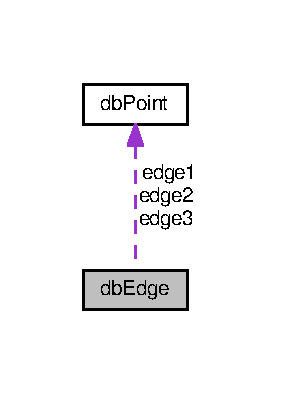
\includegraphics[width=135pt]{structdbEdge__coll__graph}
\end{center}
\end{figure}
\subsection*{Campos de Dados}
\begin{DoxyCompactItemize}
\item 
\hyperlink{structdbPoint}{db\+Point} $\ast$ \hyperlink{structdbEdge_a0886057d00d21df9488a339b5dd15f4a}{edge1}
\item 
\hyperlink{structdbPoint}{db\+Point} $\ast$ \hyperlink{structdbEdge_a2b83dba0cd9a8636cdb2eee74a1c6573}{edge2}
\item 
\hyperlink{structdbPoint}{db\+Point} $\ast$ \hyperlink{structdbEdge_a36b1358ac94b0054e16334e6727b6d2a}{edge3}
\end{DoxyCompactItemize}


\subsection{Descrição Detalhada}
Declaração da estrutura aresta, onde esta contém três ponteiros do tipo \char`\"{}db\+Point\char`\"{} arestas que compõem um triângulo que apontam para edge1, edge2 e edge3; 

\subsection{Campos}
\index{db\+Edge@{db\+Edge}!edge1@{edge1}}
\index{edge1@{edge1}!db\+Edge@{db\+Edge}}
\subsubsection[{\texorpdfstring{edge1}{edge1}}]{\setlength{\rightskip}{0pt plus 5cm}{\bf db\+Point}$\ast$ edge1}\hypertarget{structdbEdge_a0886057d00d21df9488a339b5dd15f4a}{}\label{structdbEdge_a0886057d00d21df9488a339b5dd15f4a}
\index{db\+Edge@{db\+Edge}!edge2@{edge2}}
\index{edge2@{edge2}!db\+Edge@{db\+Edge}}
\subsubsection[{\texorpdfstring{edge2}{edge2}}]{\setlength{\rightskip}{0pt plus 5cm}{\bf db\+Point}$\ast$ edge2}\hypertarget{structdbEdge_a2b83dba0cd9a8636cdb2eee74a1c6573}{}\label{structdbEdge_a2b83dba0cd9a8636cdb2eee74a1c6573}
\index{db\+Edge@{db\+Edge}!edge3@{edge3}}
\index{edge3@{edge3}!db\+Edge@{db\+Edge}}
\subsubsection[{\texorpdfstring{edge3}{edge3}}]{\setlength{\rightskip}{0pt plus 5cm}{\bf db\+Point}$\ast$ edge3}\hypertarget{structdbEdge_a36b1358ac94b0054e16334e6727b6d2a}{}\label{structdbEdge_a36b1358ac94b0054e16334e6727b6d2a}


A documentação para esta estrutura foi gerada a partir do seguinte arquivo\+:\begin{DoxyCompactItemize}
\item 
\hyperlink{lib_8h}{lib.\+h}\end{DoxyCompactItemize}

\hypertarget{structdbFace}{}\section{Referência da Estrutura db\+Face}
\label{structdbFace}\index{db\+Face@{db\+Face}}


{\ttfamily \#include $<$lib.\+h$>$}



Diagrama de colaboração para db\+Face\+:
\nopagebreak
\begin{figure}[H]
\begin{center}
\leavevmode
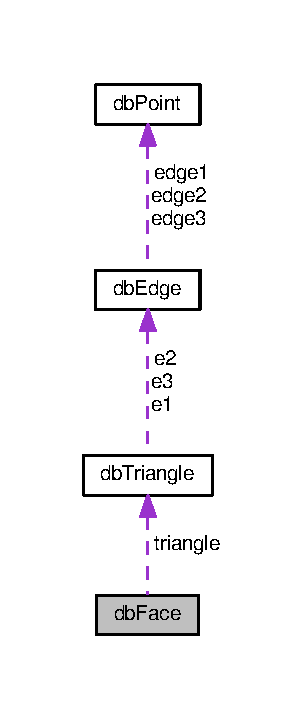
\includegraphics[width=146pt]{structdbFace__coll__graph}
\end{center}
\end{figure}
\subsection*{Campos de Dados}
\begin{DoxyCompactItemize}
\item 
\hyperlink{structdbTriangle}{db\+Triangle} \hyperlink{structdbFace_a1600f7dbf1d0654be251c20dc049837c}{triangle}
\item 
G\+S\+List $\ast$ \hyperlink{structdbFace_a6018f19ec73ee7aa43998a9d763c635f}{surfaces}
\end{DoxyCompactItemize}


\subsection{Descrição Detalhada}
Declaração da estrutura face, onde \char`\"{}triangle\char`\"{} é uma triângulo do tipo \char`\"{}db\+Triangle\char`\"{} que no caso, é um triângulo que compõe uma face. 

\subsection{Campos}
\index{db\+Face@{db\+Face}!surfaces@{surfaces}}
\index{surfaces@{surfaces}!db\+Face@{db\+Face}}
\subsubsection[{\texorpdfstring{surfaces}{surfaces}}]{\setlength{\rightskip}{0pt plus 5cm}G\+S\+List$\ast$ surfaces}\hypertarget{structdbFace_a6018f19ec73ee7aa43998a9d763c635f}{}\label{structdbFace_a6018f19ec73ee7aa43998a9d763c635f}
\index{db\+Face@{db\+Face}!triangle@{triangle}}
\index{triangle@{triangle}!db\+Face@{db\+Face}}
\subsubsection[{\texorpdfstring{triangle}{triangle}}]{\setlength{\rightskip}{0pt plus 5cm}{\bf db\+Triangle} triangle}\hypertarget{structdbFace_a1600f7dbf1d0654be251c20dc049837c}{}\label{structdbFace_a1600f7dbf1d0654be251c20dc049837c}


A documentação para esta estrutura foi gerada a partir do seguinte arquivo\+:\begin{DoxyCompactItemize}
\item 
\hyperlink{lib_8h}{lib.\+h}\end{DoxyCompactItemize}

\hypertarget{structdbPoint}{}\section{Referência da Estrutura db\+Point}
\label{structdbPoint}\index{db\+Point@{db\+Point}}


{\ttfamily \#include $<$lib.\+h$>$}

\subsection*{Campos de Dados}
\begin{DoxyCompactItemize}
\item 
Gts\+Object \hyperlink{structdbPoint_a4c9ad028a3c5d740f1fc0b15669c1c0f}{object}
\item 
double \hyperlink{structdbPoint_af88b946fb90d5f08b5fb740c70e98c10}{x}
\item 
double \hyperlink{structdbPoint_ab927965981178aa1fba979a37168db2a}{y}
\item 
double \hyperlink{structdbPoint_ab3e6ed577a7c669c19de1f9c1b46c872}{z}
\end{DoxyCompactItemize}


\subsection{Descrição Detalhada}
Declaração da estrutura ponto, onde esta contém os elementos x, y e z referentes ao espaço tridimensional; 

\subsection{Campos}
\index{db\+Point@{db\+Point}!object@{object}}
\index{object@{object}!db\+Point@{db\+Point}}
\subsubsection[{\texorpdfstring{object}{object}}]{\setlength{\rightskip}{0pt plus 5cm}Gts\+Object object}\hypertarget{structdbPoint_a4c9ad028a3c5d740f1fc0b15669c1c0f}{}\label{structdbPoint_a4c9ad028a3c5d740f1fc0b15669c1c0f}
\index{db\+Point@{db\+Point}!x@{x}}
\index{x@{x}!db\+Point@{db\+Point}}
\subsubsection[{\texorpdfstring{x}{x}}]{\setlength{\rightskip}{0pt plus 5cm}double x}\hypertarget{structdbPoint_af88b946fb90d5f08b5fb740c70e98c10}{}\label{structdbPoint_af88b946fb90d5f08b5fb740c70e98c10}
\index{db\+Point@{db\+Point}!y@{y}}
\index{y@{y}!db\+Point@{db\+Point}}
\subsubsection[{\texorpdfstring{y}{y}}]{\setlength{\rightskip}{0pt plus 5cm}double y}\hypertarget{structdbPoint_ab927965981178aa1fba979a37168db2a}{}\label{structdbPoint_ab927965981178aa1fba979a37168db2a}
\index{db\+Point@{db\+Point}!z@{z}}
\index{z@{z}!db\+Point@{db\+Point}}
\subsubsection[{\texorpdfstring{z}{z}}]{\setlength{\rightskip}{0pt plus 5cm}double z}\hypertarget{structdbPoint_ab3e6ed577a7c669c19de1f9c1b46c872}{}\label{structdbPoint_ab3e6ed577a7c669c19de1f9c1b46c872}


A documentação para esta estrutura foi gerada a partir do seguinte arquivo\+:\begin{DoxyCompactItemize}
\item 
\hyperlink{lib_8h}{lib.\+h}\end{DoxyCompactItemize}

\hypertarget{structdbSegment}{}\section{Referência da Estrutura db\+Segment}
\label{structdbSegment}\index{db\+Segment@{db\+Segment}}


{\ttfamily \#include $<$lib.\+h$>$}



Diagrama de colaboração para db\+Segment\+:\nopagebreak
\begin{figure}[H]
\begin{center}
\leavevmode
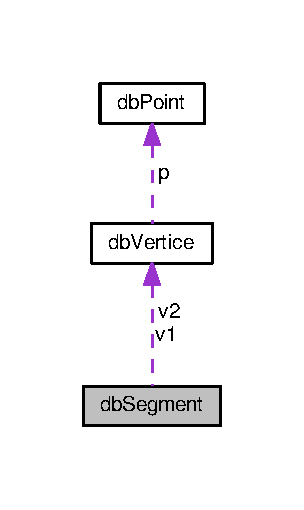
\includegraphics[width=146pt]{structdbSegment__coll__graph}
\end{center}
\end{figure}
\subsection*{Campos de Dados}
\begin{DoxyCompactItemize}
\item 
Gts\+Object \hyperlink{structdbSegment_a4c9ad028a3c5d740f1fc0b15669c1c0f}{object}
\item 
\hyperlink{structdbVertice}{db\+Vertice} $\ast$ \hyperlink{structdbSegment_ac54d355714c397af2824dfa3743b0059}{v1}
\item 
\hyperlink{structdbVertice}{db\+Vertice} $\ast$ \hyperlink{structdbSegment_a63dc8509dabff387725bbdc284734f6a}{v2}
\end{DoxyCompactItemize}


\subsection{Descrição Detalhada}
Declaração da estrutura segmento, onde esta contém dois ponteiros do tipo \char`\"{}db\+Vertice\char`\"{} que são os vértices de um segmento de reta; 

\subsection{Campos}
\index{db\+Segment@{db\+Segment}!object@{object}}
\index{object@{object}!db\+Segment@{db\+Segment}}
\subsubsection[{\texorpdfstring{object}{object}}]{\setlength{\rightskip}{0pt plus 5cm}Gts\+Object object}\hypertarget{structdbSegment_a4c9ad028a3c5d740f1fc0b15669c1c0f}{}\label{structdbSegment_a4c9ad028a3c5d740f1fc0b15669c1c0f}
\index{db\+Segment@{db\+Segment}!v1@{v1}}
\index{v1@{v1}!db\+Segment@{db\+Segment}}
\subsubsection[{\texorpdfstring{v1}{v1}}]{\setlength{\rightskip}{0pt plus 5cm}{\bf db\+Vertice}$\ast$ v1}\hypertarget{structdbSegment_ac54d355714c397af2824dfa3743b0059}{}\label{structdbSegment_ac54d355714c397af2824dfa3743b0059}
\index{db\+Segment@{db\+Segment}!v2@{v2}}
\index{v2@{v2}!db\+Segment@{db\+Segment}}
\subsubsection[{\texorpdfstring{v2}{v2}}]{\setlength{\rightskip}{0pt plus 5cm}{\bf db\+Vertice}$\ast$ v2}\hypertarget{structdbSegment_a63dc8509dabff387725bbdc284734f6a}{}\label{structdbSegment_a63dc8509dabff387725bbdc284734f6a}


A documentação para esta estrutura foi gerada a partir do seguinte arquivo\+:\begin{DoxyCompactItemize}
\item 
\hyperlink{lib_8h}{lib.\+h}\end{DoxyCompactItemize}

\hypertarget{structdbSurface}{}\section{Referência da Estrutura db\+Surface}
\label{structdbSurface}\index{db\+Surface@{db\+Surface}}


{\ttfamily \#include $<$lib.\+h$>$}

\subsection*{Campos de Dados}
\begin{DoxyCompactItemize}
\item 
Gts\+Object \hyperlink{structdbSurface_a4c9ad028a3c5d740f1fc0b15669c1c0f}{object}
\item 
G\+Hash\+Table $\ast$ \hyperlink{structdbSurface_a2491590bd6d18542d6fab3090c43f646}{faces}
\item 
Gts\+Face\+Class $\ast$ \hyperlink{structdbSurface_a9bdc080583f3916fa54dff0733e84c22}{face\+\_\+class}
\item 
Gts\+Edge\+Class $\ast$ \hyperlink{structdbSurface_aac3a854484328efcd046bed6b836ca03}{edge\+\_\+class}
\item 
Gts\+Vertex\+Class $\ast$ \hyperlink{structdbSurface_a40aba9c5621bf74c8d649089e1a82529}{vertex\+\_\+class}
\item 
gboolean \hyperlink{structdbSurface_a91e9416b378907785e1867c96a71e302}{keep\+\_\+faces}
\end{DoxyCompactItemize}


\subsection{Campos}
\index{db\+Surface@{db\+Surface}!edge\+\_\+class@{edge\+\_\+class}}
\index{edge\+\_\+class@{edge\+\_\+class}!db\+Surface@{db\+Surface}}
\subsubsection[{\texorpdfstring{edge\+\_\+class}{edge_class}}]{\setlength{\rightskip}{0pt plus 5cm}Gts\+Edge\+Class$\ast$ edge\+\_\+class}\hypertarget{structdbSurface_aac3a854484328efcd046bed6b836ca03}{}\label{structdbSurface_aac3a854484328efcd046bed6b836ca03}
\index{db\+Surface@{db\+Surface}!face\+\_\+class@{face\+\_\+class}}
\index{face\+\_\+class@{face\+\_\+class}!db\+Surface@{db\+Surface}}
\subsubsection[{\texorpdfstring{face\+\_\+class}{face_class}}]{\setlength{\rightskip}{0pt plus 5cm}Gts\+Face\+Class$\ast$ face\+\_\+class}\hypertarget{structdbSurface_a9bdc080583f3916fa54dff0733e84c22}{}\label{structdbSurface_a9bdc080583f3916fa54dff0733e84c22}
\index{db\+Surface@{db\+Surface}!faces@{faces}}
\index{faces@{faces}!db\+Surface@{db\+Surface}}
\subsubsection[{\texorpdfstring{faces}{faces}}]{\setlength{\rightskip}{0pt plus 5cm}G\+Hash\+Table$\ast$ faces}\hypertarget{structdbSurface_a2491590bd6d18542d6fab3090c43f646}{}\label{structdbSurface_a2491590bd6d18542d6fab3090c43f646}
\index{db\+Surface@{db\+Surface}!keep\+\_\+faces@{keep\+\_\+faces}}
\index{keep\+\_\+faces@{keep\+\_\+faces}!db\+Surface@{db\+Surface}}
\subsubsection[{\texorpdfstring{keep\+\_\+faces}{keep_faces}}]{\setlength{\rightskip}{0pt plus 5cm}gboolean keep\+\_\+faces}\hypertarget{structdbSurface_a91e9416b378907785e1867c96a71e302}{}\label{structdbSurface_a91e9416b378907785e1867c96a71e302}
\index{db\+Surface@{db\+Surface}!object@{object}}
\index{object@{object}!db\+Surface@{db\+Surface}}
\subsubsection[{\texorpdfstring{object}{object}}]{\setlength{\rightskip}{0pt plus 5cm}Gts\+Object object}\hypertarget{structdbSurface_a4c9ad028a3c5d740f1fc0b15669c1c0f}{}\label{structdbSurface_a4c9ad028a3c5d740f1fc0b15669c1c0f}
\index{db\+Surface@{db\+Surface}!vertex\+\_\+class@{vertex\+\_\+class}}
\index{vertex\+\_\+class@{vertex\+\_\+class}!db\+Surface@{db\+Surface}}
\subsubsection[{\texorpdfstring{vertex\+\_\+class}{vertex_class}}]{\setlength{\rightskip}{0pt plus 5cm}Gts\+Vertex\+Class$\ast$ vertex\+\_\+class}\hypertarget{structdbSurface_a40aba9c5621bf74c8d649089e1a82529}{}\label{structdbSurface_a40aba9c5621bf74c8d649089e1a82529}


A documentação para esta estrutura foi gerada a partir do seguinte arquivo\+:\begin{DoxyCompactItemize}
\item 
\hyperlink{lib_8h}{lib.\+h}\end{DoxyCompactItemize}

\hypertarget{structdbTriangle}{}\section{Referência da Estrutura db\+Triangle}
\label{structdbTriangle}\index{db\+Triangle@{db\+Triangle}}


{\ttfamily \#include $<$lib.\+h$>$}



Diagrama de colaboração para db\+Triangle\+:\nopagebreak
\begin{figure}[H]
\begin{center}
\leavevmode
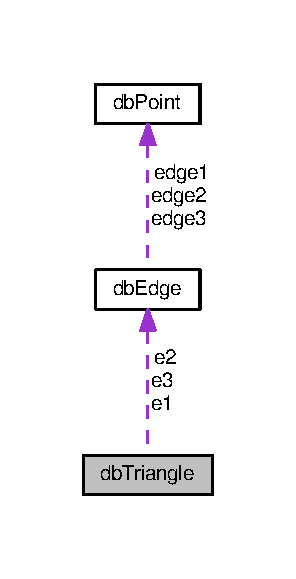
\includegraphics[width=142pt]{structdbTriangle__coll__graph}
\end{center}
\end{figure}
\subsection*{Campos de Dados}
\begin{DoxyCompactItemize}
\item 
Gts\+Object \hyperlink{structdbTriangle_a4c9ad028a3c5d740f1fc0b15669c1c0f}{object}
\item 
\hyperlink{structdbEdge}{db\+Edge} $\ast$ \hyperlink{structdbTriangle_a038c41bf0720b16e63178f1915b0e455}{e1}
\item 
\hyperlink{structdbEdge}{db\+Edge} $\ast$ \hyperlink{structdbTriangle_a0b0a41cfaeb4cee2ad5d8578359c61c8}{e2}
\item 
\hyperlink{structdbEdge}{db\+Edge} $\ast$ \hyperlink{structdbTriangle_a5e66d5366546f4c9cd75c879bd054efd}{e3}
\end{DoxyCompactItemize}


\subsection{Descrição Detalhada}
Declaração da estrutura triângulo, onde \char`\"{}e\char`\"{} é uma aresta, e esta estrutura contém três arestas do tipo \char`\"{}db\+Edge\char`\"{} arestas que compõem um triângulo. Esses ponteiros apontam para e1, e2 e e3; 

\subsection{Campos}
\index{db\+Triangle@{db\+Triangle}!e1@{e1}}
\index{e1@{e1}!db\+Triangle@{db\+Triangle}}
\subsubsection[{\texorpdfstring{e1}{e1}}]{\setlength{\rightskip}{0pt plus 5cm}{\bf db\+Edge}$\ast$ e1}\hypertarget{structdbTriangle_a038c41bf0720b16e63178f1915b0e455}{}\label{structdbTriangle_a038c41bf0720b16e63178f1915b0e455}
\index{db\+Triangle@{db\+Triangle}!e2@{e2}}
\index{e2@{e2}!db\+Triangle@{db\+Triangle}}
\subsubsection[{\texorpdfstring{e2}{e2}}]{\setlength{\rightskip}{0pt plus 5cm}{\bf db\+Edge}$\ast$ e2}\hypertarget{structdbTriangle_a0b0a41cfaeb4cee2ad5d8578359c61c8}{}\label{structdbTriangle_a0b0a41cfaeb4cee2ad5d8578359c61c8}
\index{db\+Triangle@{db\+Triangle}!e3@{e3}}
\index{e3@{e3}!db\+Triangle@{db\+Triangle}}
\subsubsection[{\texorpdfstring{e3}{e3}}]{\setlength{\rightskip}{0pt plus 5cm}{\bf db\+Edge}$\ast$ e3}\hypertarget{structdbTriangle_a5e66d5366546f4c9cd75c879bd054efd}{}\label{structdbTriangle_a5e66d5366546f4c9cd75c879bd054efd}
\index{db\+Triangle@{db\+Triangle}!object@{object}}
\index{object@{object}!db\+Triangle@{db\+Triangle}}
\subsubsection[{\texorpdfstring{object}{object}}]{\setlength{\rightskip}{0pt plus 5cm}Gts\+Object object}\hypertarget{structdbTriangle_a4c9ad028a3c5d740f1fc0b15669c1c0f}{}\label{structdbTriangle_a4c9ad028a3c5d740f1fc0b15669c1c0f}


A documentação para esta estrutura foi gerada a partir do seguinte arquivo\+:\begin{DoxyCompactItemize}
\item 
\hyperlink{lib_8h}{lib.\+h}\end{DoxyCompactItemize}

\hypertarget{structdbVertice}{}\section{Referência da Estrutura db\+Vertice}
\label{structdbVertice}\index{db\+Vertice@{db\+Vertice}}


{\ttfamily \#include $<$lib.\+h$>$}



Diagrama de colaboração para db\+Vertice\+:\nopagebreak
\begin{figure}[H]
\begin{center}
\leavevmode
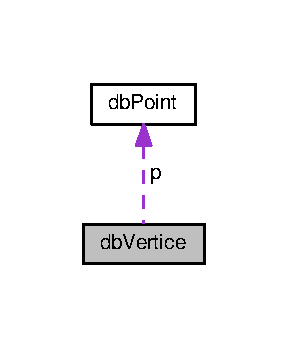
\includegraphics[width=138pt]{structdbVertice__coll__graph}
\end{center}
\end{figure}
\subsection*{Campos de Dados}
\begin{DoxyCompactItemize}
\item 
\hyperlink{structdbPoint}{db\+Point} \hyperlink{structdbVertice_a03ab875eb2041f01ba2b5b86d413896b}{p}
\item 
G\+S\+List $\ast$ \hyperlink{structdbVertice_a0ae9e8feccea4307d768c5c1463f4d28}{segments}
\end{DoxyCompactItemize}


\subsection{Descrição Detalhada}
Declaração da estrutura vértice, onde esta contém um ponteiro do tipo \char`\"{}db\+Point\char`\"{} que é o ponto do vértice. 

\subsection{Campos}
\index{db\+Vertice@{db\+Vertice}!p@{p}}
\index{p@{p}!db\+Vertice@{db\+Vertice}}
\subsubsection[{\texorpdfstring{p}{p}}]{\setlength{\rightskip}{0pt plus 5cm}{\bf db\+Point} p}\hypertarget{structdbVertice_a03ab875eb2041f01ba2b5b86d413896b}{}\label{structdbVertice_a03ab875eb2041f01ba2b5b86d413896b}
\index{db\+Vertice@{db\+Vertice}!segments@{segments}}
\index{segments@{segments}!db\+Vertice@{db\+Vertice}}
\subsubsection[{\texorpdfstring{segments}{segments}}]{\setlength{\rightskip}{0pt plus 5cm}G\+S\+List$\ast$ segments}\hypertarget{structdbVertice_a0ae9e8feccea4307d768c5c1463f4d28}{}\label{structdbVertice_a0ae9e8feccea4307d768c5c1463f4d28}


A documentação para esta estrutura foi gerada a partir do seguinte arquivo\+:\begin{DoxyCompactItemize}
\item 
\hyperlink{lib_8h}{lib.\+h}\end{DoxyCompactItemize}

\chapter{Arquivos}
\hypertarget{code_8c}{}\section{Referência do Arquivo code.\+c}
\label{code_8c}\index{code.\+c@{code.\+c}}
{\ttfamily \#include $<$stdio.\+h$>$}\\*
{\ttfamily \#include \char`\"{}lib.\+h\char`\"{}}\\*
Gráfico de dependência de inclusões para code.\+c\+:
\nopagebreak
\begin{figure}[H]
\begin{center}
\leavevmode
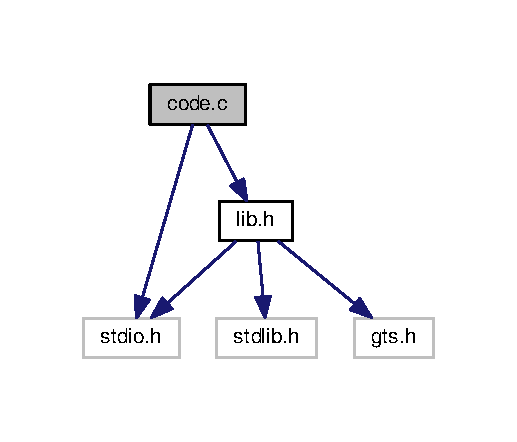
\includegraphics[width=248pt]{code_8c__incl}
\end{center}
\end{figure}
\subsection*{Funções}
\begin{DoxyCompactItemize}
\item 
int \hyperlink{code_8c_a5845bd661567fddf74a5bff297369413}{function} (int var)
\item 
int \hyperlink{code_8c_ae66f6b31b5ad750f1fe042a706a4e3d4}{main} ()
\begin{DoxyCompactList}\small\item\em Descrição em breve. \end{DoxyCompactList}\end{DoxyCompactItemize}


\subsection{Funções}
\index{code.\+c@{code.\+c}!function@{function}}
\index{function@{function}!code.\+c@{code.\+c}}
\subsubsection[{\texorpdfstring{function(int var)}{function(int var)}}]{\setlength{\rightskip}{0pt plus 5cm}int function (
\begin{DoxyParamCaption}
\item[{int}]{var}
\end{DoxyParamCaption}
)}\hypertarget{code_8c_a5845bd661567fddf74a5bff297369413}{}\label{code_8c_a5845bd661567fddf74a5bff297369413}
Test function $<$A variavel \char`\"{}var\char`\"{} recebe ela mesmo vezes 2 \index{code.\+c@{code.\+c}!main@{main}}
\index{main@{main}!code.\+c@{code.\+c}}
\subsubsection[{\texorpdfstring{main()}{main()}}]{\setlength{\rightskip}{0pt plus 5cm}int main (
\begin{DoxyParamCaption}
{}
\end{DoxyParamCaption}
)}\hypertarget{code_8c_ae66f6b31b5ad750f1fe042a706a4e3d4}{}\label{code_8c_ae66f6b31b5ad750f1fe042a706a4e3d4}


Descrição em breve. 

Função main $<$ Detailed description after the member 
\hypertarget{COMO_01COMPILAR_8txt}{}\section{Referência do Arquivo C\+O\+MO C\+O\+M\+P\+I\+L\+A\+R.\+txt}
\label{COMO_01COMPILAR_8txt}\index{C\+O\+M\+O C\+O\+M\+P\+I\+L\+A\+R.\+txt@{C\+O\+M\+O C\+O\+M\+P\+I\+L\+A\+R.\+txt}}

\hypertarget{lib_8h}{}\section{Referência do Arquivo lib.\+h}
\label{lib_8h}\index{lib.\+h@{lib.\+h}}
{\ttfamily \#include $<$stdio.\+h$>$}\\*
{\ttfamily \#include $<$stdlib.\+h$>$}\\*
{\ttfamily \#include $<$gts.\+h$>$}\\*
Gráfico de dependência de inclusões para lib.\+h\+:
\nopagebreak
\begin{figure}[H]
\begin{center}
\leavevmode
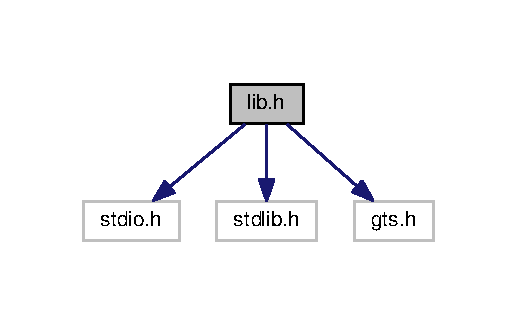
\includegraphics[width=248pt]{lib_8h__incl}
\end{center}
\end{figure}
Este grafo mostra quais arquivos estão direta ou indiretamente relacionados com este arquivo\+:
\nopagebreak
\begin{figure}[H]
\begin{center}
\leavevmode
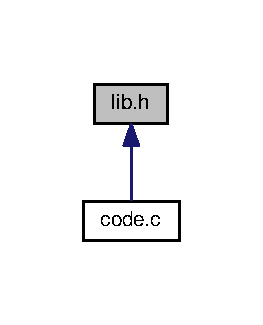
\includegraphics[width=126pt]{lib_8h__dep__incl}
\end{center}
\end{figure}
\subsection*{Estruturas de Dados}
\begin{DoxyCompactItemize}
\item 
struct \hyperlink{structdbPoint}{db\+Point}
\item 
struct \hyperlink{structdbVertice}{db\+Vertice}
\item 
struct \hyperlink{structdbSegment}{db\+Segment}
\item 
struct \hyperlink{structdbEdge}{db\+Edge}
\item 
struct \hyperlink{structdbTriangle}{db\+Triangle}
\item 
struct \hyperlink{structdbFace}{db\+Face}
\item 
struct \hyperlink{structdbSurface}{db\+Surface}
\end{DoxyCompactItemize}
\subsection*{Definições de Tipos}
\begin{DoxyCompactItemize}
\item 
typedef struct \hyperlink{structdbPoint}{db\+Point} \hyperlink{lib_8h_a6e636f3c7274f92304d9d27a69113609}{db\+Point}
\item 
typedef struct \hyperlink{structdbVertice}{db\+Vertice} \hyperlink{lib_8h_add1784c66680084dfa0471b2219ba2ce}{db\+Vertice}
\item 
typedef struct \hyperlink{structdbSegment}{db\+Segment} \hyperlink{lib_8h_af8d52ab5a8bc633defa9f0173bfff4ec}{db\+Segment}
\item 
typedef struct \hyperlink{structdbEdge}{db\+Edge} \hyperlink{lib_8h_a13cbf2b8bc3f4c8dbcec2cc7829af1f7}{db\+Edge}
\item 
typedef struct \hyperlink{structdbTriangle}{db\+Triangle} \hyperlink{lib_8h_a886a817b2f33af3a8d4127e64872a0ea}{db\+Triangle}
\item 
typedef struct \hyperlink{structdbFace}{db\+Face} \hyperlink{lib_8h_ad6a7a07c077313f533d08e35e4fb7dae}{db\+Face}
\item 
typedef struct \hyperlink{structdbSurface}{db\+Surface} \hyperlink{lib_8h_a746afe6b815c56aed82814c8986b8578}{db\+Surface}
\end{DoxyCompactItemize}


\subsection{Definições dos tipos}
\index{lib.\+h@{lib.\+h}!db\+Edge@{db\+Edge}}
\index{db\+Edge@{db\+Edge}!lib.\+h@{lib.\+h}}
\subsubsection[{\texorpdfstring{db\+Edge}{dbEdge}}]{\setlength{\rightskip}{0pt plus 5cm}typedef struct {\bf db\+Edge} {\bf db\+Edge}}\hypertarget{lib_8h_a13cbf2b8bc3f4c8dbcec2cc7829af1f7}{}\label{lib_8h_a13cbf2b8bc3f4c8dbcec2cc7829af1f7}
Declaração da estrutura aresta, onde esta contém três ponteiros do tipo \char`\"{}db\+Point\char`\"{} arestas que compõem um triângulo que apontam para edge1, edge2 e edge3; \index{lib.\+h@{lib.\+h}!db\+Face@{db\+Face}}
\index{db\+Face@{db\+Face}!lib.\+h@{lib.\+h}}
\subsubsection[{\texorpdfstring{db\+Face}{dbFace}}]{\setlength{\rightskip}{0pt plus 5cm}typedef struct {\bf db\+Face} {\bf db\+Face}}\hypertarget{lib_8h_ad6a7a07c077313f533d08e35e4fb7dae}{}\label{lib_8h_ad6a7a07c077313f533d08e35e4fb7dae}
Declaração da estrutura face, onde \char`\"{}triangle\char`\"{} é uma triângulo do tipo \char`\"{}db\+Triangle\char`\"{} que no caso, é um triângulo que compõe uma face. \index{lib.\+h@{lib.\+h}!db\+Point@{db\+Point}}
\index{db\+Point@{db\+Point}!lib.\+h@{lib.\+h}}
\subsubsection[{\texorpdfstring{db\+Point}{dbPoint}}]{\setlength{\rightskip}{0pt plus 5cm}typedef struct {\bf db\+Point} {\bf db\+Point}}\hypertarget{lib_8h_a6e636f3c7274f92304d9d27a69113609}{}\label{lib_8h_a6e636f3c7274f92304d9d27a69113609}
Declaração da estrutura ponto, onde esta contém os elementos x, y e z referentes ao espaço tridimensional; \index{lib.\+h@{lib.\+h}!db\+Segment@{db\+Segment}}
\index{db\+Segment@{db\+Segment}!lib.\+h@{lib.\+h}}
\subsubsection[{\texorpdfstring{db\+Segment}{dbSegment}}]{\setlength{\rightskip}{0pt plus 5cm}typedef struct {\bf db\+Segment} {\bf db\+Segment}}\hypertarget{lib_8h_af8d52ab5a8bc633defa9f0173bfff4ec}{}\label{lib_8h_af8d52ab5a8bc633defa9f0173bfff4ec}
Declaração da estrutura segmento, onde esta contém dois ponteiros do tipo \char`\"{}db\+Vertice\char`\"{} que são os vértices de um segmento de reta; \index{lib.\+h@{lib.\+h}!db\+Surface@{db\+Surface}}
\index{db\+Surface@{db\+Surface}!lib.\+h@{lib.\+h}}
\subsubsection[{\texorpdfstring{db\+Surface}{dbSurface}}]{\setlength{\rightskip}{0pt plus 5cm}typedef struct {\bf db\+Surface} {\bf db\+Surface}}\hypertarget{lib_8h_a746afe6b815c56aed82814c8986b8578}{}\label{lib_8h_a746afe6b815c56aed82814c8986b8578}
\index{lib.\+h@{lib.\+h}!db\+Triangle@{db\+Triangle}}
\index{db\+Triangle@{db\+Triangle}!lib.\+h@{lib.\+h}}
\subsubsection[{\texorpdfstring{db\+Triangle}{dbTriangle}}]{\setlength{\rightskip}{0pt plus 5cm}typedef struct {\bf db\+Triangle} {\bf db\+Triangle}}\hypertarget{lib_8h_a886a817b2f33af3a8d4127e64872a0ea}{}\label{lib_8h_a886a817b2f33af3a8d4127e64872a0ea}
Declaração da estrutura triângulo, onde \char`\"{}e\char`\"{} é uma aresta, e esta estrutura contém três arestas do tipo \char`\"{}db\+Edge\char`\"{} arestas que compõem um triângulo. Esses ponteiros apontam para e1, e2 e e3; \index{lib.\+h@{lib.\+h}!db\+Vertice@{db\+Vertice}}
\index{db\+Vertice@{db\+Vertice}!lib.\+h@{lib.\+h}}
\subsubsection[{\texorpdfstring{db\+Vertice}{dbVertice}}]{\setlength{\rightskip}{0pt plus 5cm}typedef struct {\bf db\+Vertice} {\bf db\+Vertice}}\hypertarget{lib_8h_add1784c66680084dfa0471b2219ba2ce}{}\label{lib_8h_add1784c66680084dfa0471b2219ba2ce}
Declaração da estrutura vértice, onde esta contém um ponteiro do tipo \char`\"{}db\+Point\char`\"{} que é o ponto do vértice. 
%--- End generated contents ---

% Index
\backmatter
\newpage
\phantomsection
\clearemptydoublepage
\addcontentsline{toc}{chapter}{Índice}
\printindex

\end{document}
